\documentclass[UTF8]{ctexbook}
\usepackage[a4paper,left=3cm,right=3cm,top=2cm]{geometry}
\usepackage{amsmath}
\usepackage{enumitem}
\usepackage{float}
\usepackage{threeparttable}
\usepackage{caption}
\usepackage{multirow}
\usepackage{graphicx}
\usepackage{subfigure}
\usepackage{fancyhdr}

\setlength\lineskiplimit{5.25bp}
\setlength\lineskip{5.25bp}


\title{浅谈深度学习}
\author{崔士强,莫环欣,朱小蕊,陈筱頔}
\date{\today}

\bibliographystyle{plain}

\begin{document}
\maketitle
\tableofcontents

\chapter{引言}
\section{深度学习简介}
深度学习是机器学习领域的一个重要分支,其概念源于人工神经网络的发展,
并受到神经科学和计算机科学的启发.
传统的机器学习方法在处理复杂的任务和大规模数据时往往面临着维度灾难和特征提取的挑战.
深度学习通过构建深层神经网络,能够自动学习数据的高级表示和特征,从而解决了这些问题.

深度学习的核心思想是通过多层次的神经网络来模拟人脑的工作方式。神经网络由多个神经元组成,
每个神经元接收来自前一层神经元的输入,并通过激活函数对这些输入进行加权求和和非线性变换.
通过多层次的神经网络结构,深度学习可以学习到数据的多层次抽象表示,从低级特征到高级语义.

深度学习的发展受益于计算能力的提升和大规模数据集的可用性。近年来,随着计算机硬件的快速发展,
特别是图形处理器(GPU)的广泛应用,深度学习模型的训练和推断速度得到了显著提升.
此外,互联网的快速发展和大数据的普及,为深度学习提供了海量的数据资源,
使得深度学习模型能够从数据中学习到更准确、更智能的模式和表示.

这里我们将从发展历程,原理,应用,展望四个方面简要介绍深度学习.
\section{各章节作者}
\begin{itemize}
    \item 第一章\qquad 崔士强
    \item 第二章\qquad 莫环欣
    \item 第三章\qquad 崔士强
    \item 第四章\qquad 陈筱頔
    \item 第五章\qquad 朱小蕊
    \item 第六章\qquad 崔士强
\end{itemize}

\let\cleardoublepage\clearpage
\chapter{深度学习的发展历程}
学习任一门知识都应该先从其历史开始,把握了历史,也就抓住了现在与未来.
\section{深度学习的起源}
\subsection{神经网络的诞生}
1943年,由神经科学家麦卡洛克(M.S.McCilloch)和数学家皮兹(W.Pitts)在《数学生物物理学公告》上发表论文《神经活动中内在思想的逻辑演算》
\footnote{McCulloch W S;;Pitts W.A logical calculus of the ideas immanent in nervous activity. 1943.[J].Bulletin of mathematical biology,1990,(1-2)} ,
建立了神经网络和数学模型,即M-P模型,最早开启通过大脑神经元解释思维过程、并通过大量非线性并行处理器模拟人类神经元的实现方法,
开创了人工神经网络的新时代,奠定了神经网络模型的基础.

1949年,加拿大著名心理学家唐纳德·赫布在《行为的组织》中提出了一种基于无监督学习的规则——海布学习规则(Hebb Rule),
模仿人类认知世界的过程建立一种“网络模型”,第一次开始考虑通过调整权值来进行算法的自我训练.

20世纪50年代末,在MP模型和海布学习规则的研究基础上,美国科学家罗森布拉特发现了一种类似于人类学习过程的学习算法-- --感知机学习,
并于1958年正式提出了由两层神经元组成的神经网络,称之为“感知器”.

1969年,“AI之父”马文·明斯基和LOGO语言的创始人西蒙·派珀特共同证明了单层感知器无法解决线性不可分问题.
\subsection{神经网络的复兴}
1982年,著名物理学家约翰·霍普菲尔德发明了Hopfield神经网络,可以模拟人类的记忆,用于优化计算和联想记忆.

1985年,G.E.Hinton和T.J.Sejnowski提出了一种随机神经网络模型——玻尔兹曼机.

1986年,深度学习之父杰弗里·辛顿提出了一种适用于多层感知器的反向传播算法——BP算法,
完美地解决了非线性分类问题,让人工神经网络再次引起了人们的广泛关注.

1989年,Hornik.K、Stinchcombe.M和White.H共同提出“万能近似定理”,说明了理论上神经网络可以近似任何函数,是深度学习最根本的理论依据;
同年,Yann LeCun构建了应用于计算机视觉问题的卷积神经网络,在论述网络结构时首次使用了“卷积”一词,“卷积神经网络”也因此得名.

1997年,德国计算机科学家于尔根·施密德胡伯(Jurgen Schmidhuber)与赛普·霍赫赖托提出了一种时间循环神经网络——长短期记忆网络(LSTM),
可作为复杂的非线性单元用于构造更大型的深度神经网络.

1998年,Yann LeCun提出了一种卷积神经网络——LeNet,适合处理图像数据,是第一个成功应用于实际问题的卷积神经网络.
\subsection{深度学习}
2006年,Geoffrey Hinton提出“深度信念网络”生成模型,可用于识别特征,分类、生成数据.同年,
“深度学习”概念由Geoffrey Hinton、Yoshua Bengio、Yann Lecun等正式提出.
\section{深度学习的发展现状}
2012年,Hinton课题组通过CNN网络AlexNet,从根本上解决了梯度消失问题,并采用GPU极大的提高了模型的运算速度,夺得了ImageNet图像识别比赛冠军.

2014年,香港中文大学汤晓鸥教授研究组开发了名为DeepID的深度学习模型,在LFW数据库上获得了99.15\%的识别率,超过了人肉眼的97.52\%的识别率,
标志着深度学习在学术研究层面上已经超过了人用肉眼的识别.

2016年3月人工智能围棋比赛,Google旗下DeepMind公司开发的AlphaGo以4:1战胜了世界围棋冠军,之后陆续与其他围棋高手对决均完胜.

2017年,基于强化学习算法的AlphaGo Zero在围棋比赛中以100:0的比分完胜其前身AlphaGo,同年,深度学习的相关算法在多个领域均取得了显著成果.

2018年6月,OpenAI开发了一种可以在未标记的文本上训练AI的技术,可以大量减少人工标注的时间.

2017年12月,社交软件Reddit上的用户“deepfakes”发布的基于深度学习技术自动化生成的视频使AI换脸技术迅速在大众视野中爆红,
随后出现了DeepFaceLab、FaceSwap、OpenFaceSwap等众多开源项目.

2022年11月30日,OpenAI推出专注于对话生成的语言模型ChatGPT,通过学习大量现成文本和对话合集,其能够根据用户的文本输入产生相应的智能回答,
将人工智能与深度学习的热度推上了一个前所未有的高峰,仅仅数月便已迭代至GPT-4(2023.3.14),目前由于伦理等问题被限制继续发展.
\let\cleardoublepage\clearpage
\chapter{深度学习的原理}
深度学习主要依赖神经网络实现,因此这里将从一个例子出发,介绍神经网络的基本原理.
\section{神经网络的结构}
\subsection{一个简单的例子}
让我们考虑这样一个例子:有三张$28\times 28$像素的手写数字的图片(图3.1)
\begin{figure}[h]
    \centering
    \subfigure
    {
        \begin{minipage}[b]{.3\linewidth}
            \centering
            
\includegraphics[width=0.6\textwidth]{3.1.png}
        \end{minipage}
    }
    \subfigure
    {
        \begin{minipage}[b]{.3\linewidth}
            \centering
            
\includegraphics[width=0.6\textwidth]{3.2.png}
        \end{minipage}
    }
    \subfigure
    {
        \begin{minipage}[b]{.3\linewidth}
            \centering
            
\includegraphics[width=0.6\textwidth]{3.3.png}
        \end{minipage}
    }
    \caption{手写数字3}
\end{figure}

虽然这三张图片的分辨率很低,而且形状各不相同(意味着它们激发的光感神经细胞大相径庭),我们的大脑仍然能识别出这都是3,而经过训练的神经网络可以做到相同的事情.
我们要做的就是模拟人脑,建立若干神经元(neuron),设定这些神经元之间的连接方式,最后使其在接受输入(在这个例子中是一张图片)后能够给出正确的输出.
下面将介绍实现这一功能的神经网络的结构
\subsection{神经网络的各个部分}
如图3.2\footnote{图源:https://www.youtube.com/watch?v=aircAruvnKk}所示,神经网络主要由神经元组成,而神经元被分为不同的层.
\begin{figure}[h]
    \centering
    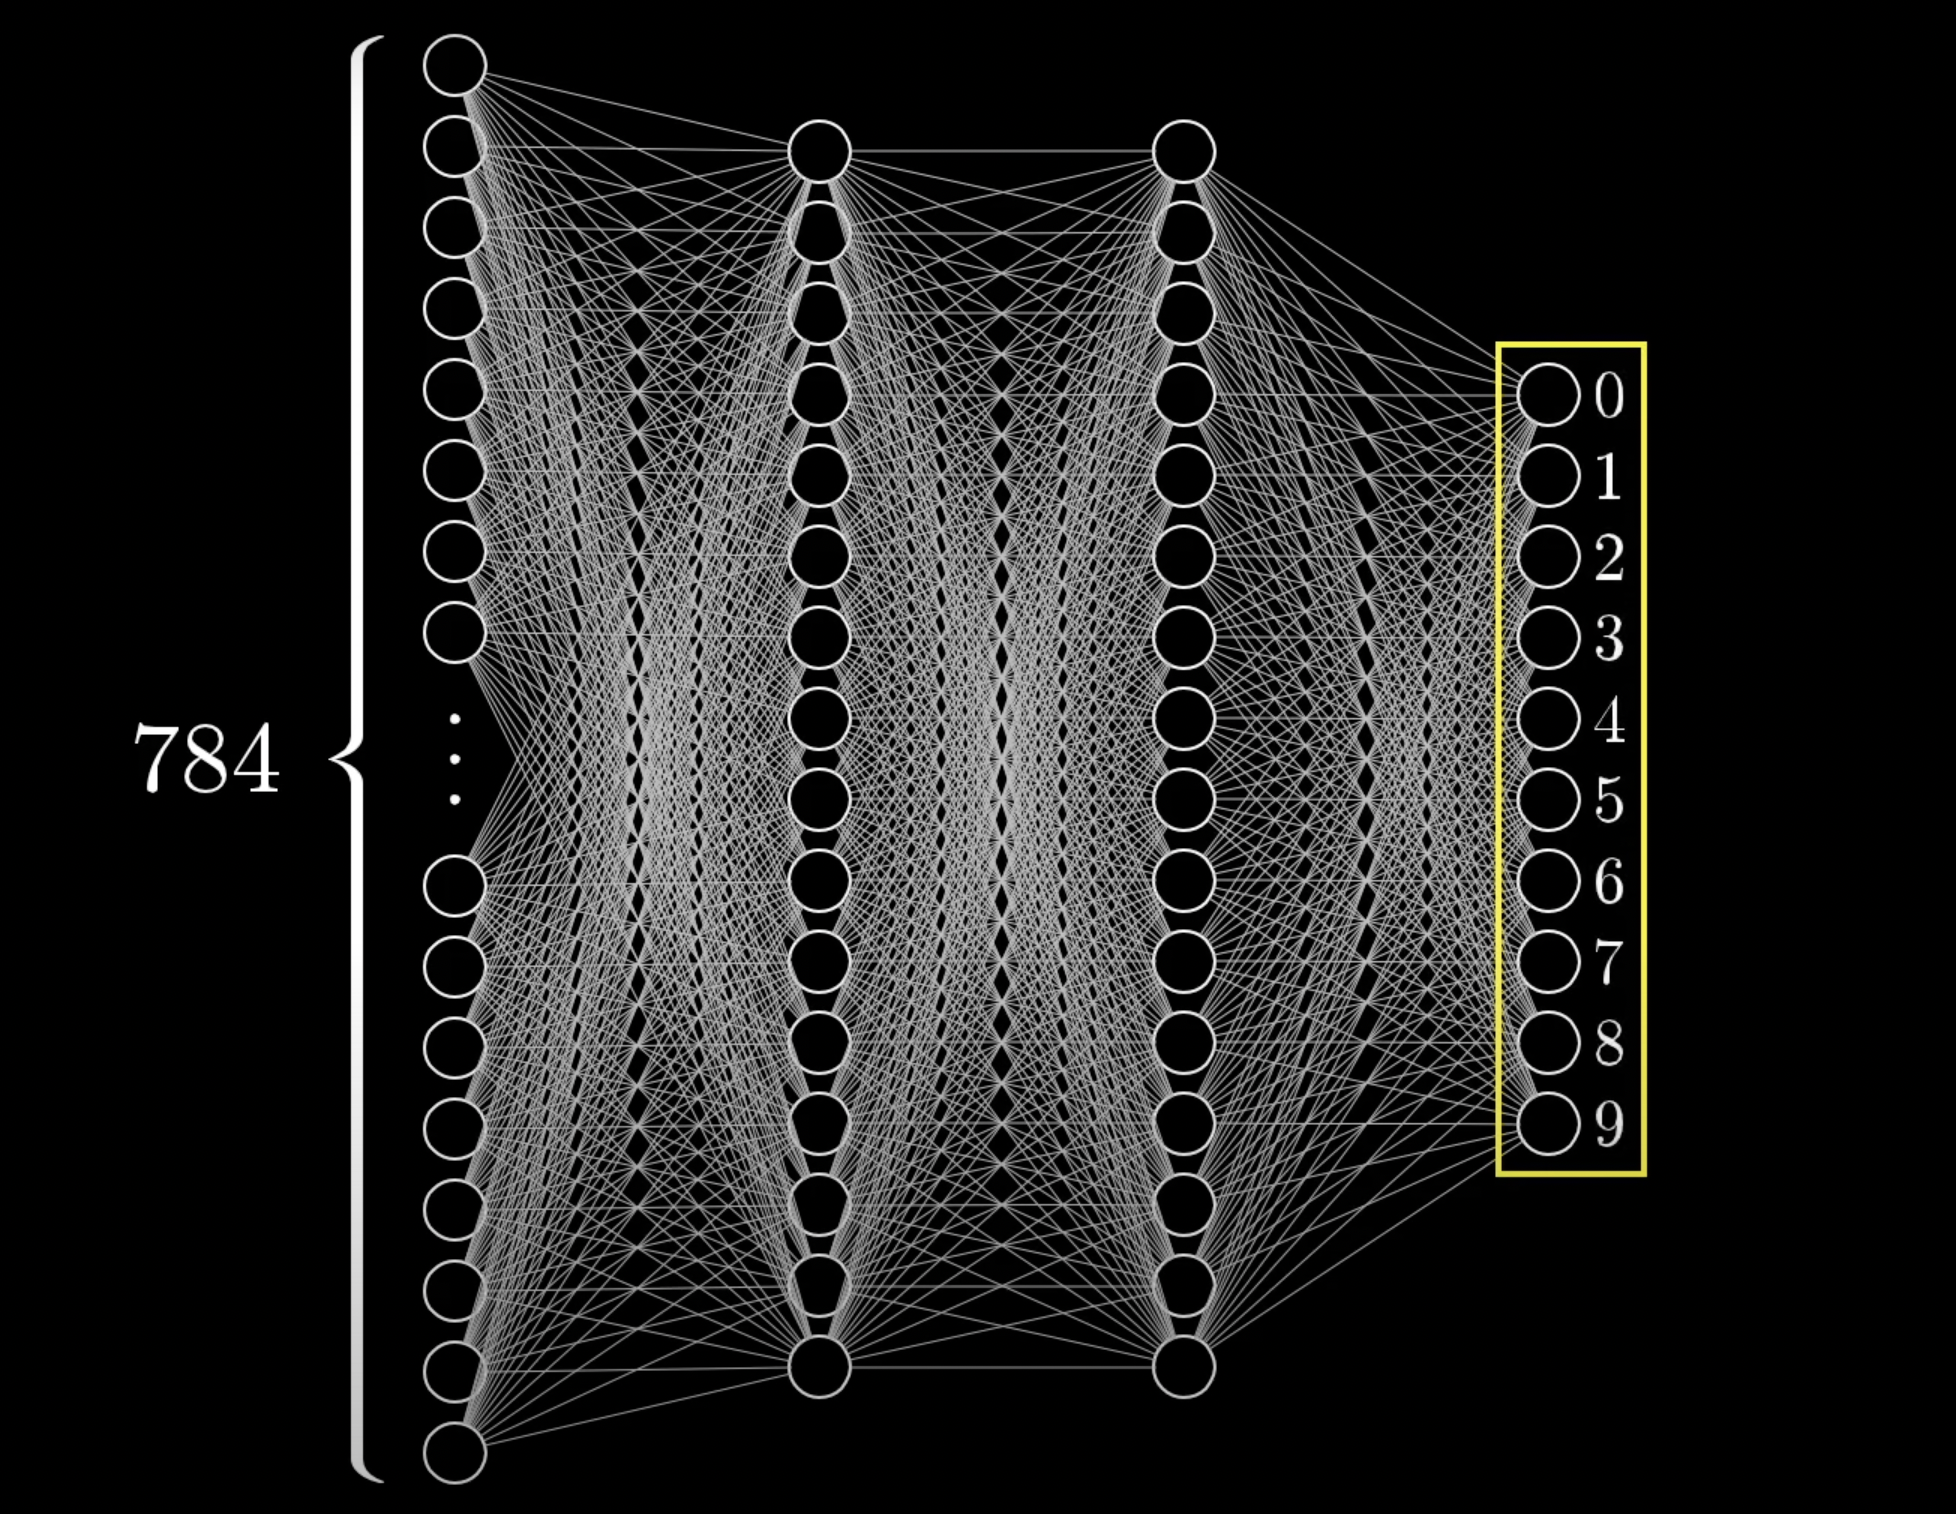
\includegraphics[width=0.4\textwidth]{neural network.png}
    \caption{神经网络示意图}
\end{figure}
\subsubsection{神经元}
上面的例子中涉及到的图片共计784个像素,对应784个神经元作为输入,每个神经元看作一个变量,其值称为激活值(activation),取值范围为$[0,1]$,
在这里即为该像素的灰度值(gray scale value), 0代表纯黑像素,1代表纯白像素.

而最后的输出结果有从0到9共计10个可能值,同样对应10个神经元,某个神经元的激发值代表神经网络认为该神经元对应的数字是正确结果的概率.
\subsubsection{层(layers)}
在这个例子中,我们可以构建一个四层的神经网络.最左侧的层为输入层(Input layer),由784个神经元组成,代表图片的信息.
最右侧的层为输出层(Output layer),由10个神经元组成,代表输出结果.中间的两层为隐藏层(Hidden layers)

在神经网络中,隐藏层的层数以及每一层的神经元都是可以调整的,这里取两个隐藏层,每层16个神经元. 在这个例子当中,这些隐藏层代表组成数字的
“部件”.例如数字8由两个圆圈组成,数字9由一个圆圈和一条线组成,等等. 我们希望倒数第二层的各个神经元能够分别代表一个“部件”,而倒数第二层
与输出层之间的连接便代表了不同部件的组合对应什么数字. 同理,第二层可以代表一些更小的“部件”。

上面所说到的原理同样适用于其他场景. 例如图像识别依赖特殊的形状来判断图片里的物体,语音识别依赖音节来判断所说的内容,等等.

接下来我们将要讨论,如何让这些神经元表示特定的“部件”.
\section{从输入到输出}
在我们输入一个样本后,神经网络通过逐层计算最后给出结果,这个过程被称为前向传播(Foward Propagation).

以第一层到第二层为例,我们提到过,在第二层中我们希望每个神经元能够表示一些基础的“部件”.这意味着我们需要关注第一层中对应这个部件的神经元. 
在神经网络中,这种“关注”是通过赋予这些神经元权重(weight)来实现的.对于第二层的第一个神经元,假设第一层神经元激发值和权重分别为$a_{i}^{(0)}$和$w_{0,i}, 1\leq i\leq 784$, 
第二层神经元激发值为$a_{2j}, 1\leq j\leq 16$, 我们可以对第一层神经元激发值的加权求和:
\[S=\sum_{i=1} ^{k}a_{i}^{(0)}w_{0,i}\]
对于这个结果,我们往往希望其达到一定门槛,此时可以添加名为偏置(bias)的常数项$b_0$. 
在这之后,我们将这个添加了偏置的求和放进一个激活函数, 常用的函数有:

\noindent Sigmoid(又称Logistic)函数:
\[\sigma(x)=\frac{1}{1+e^{-x}}\]
以及ReLU(Rectified Linear Unit)函数\footnote{由于更容易训练,目前的神经网络使用这个函数较多}:
\[ReLU(x)=\max \{0,x\}\]
等等.

这样,我们便得到了第二层第一个神经元激发值的表达式(激活函数以Sigmoid函数为例):
\[a_0^{(1)}=\sigma\left(\sum_{i=1} ^{n}a_{i}^{(0)}w_{0,i}+b_0\right)\]
对于整个第二层,我们可以写成矩阵运算的形式:
\[
\begin{bmatrix}
    a_0^{(1)} \\
    a_1^{(1)} \\
    \vdots \\
    a_k^{(1)} \\
\end{bmatrix}
=
\sigma \left(
\begin{bmatrix}
    w_{0,0} & w_{0,1} & \cdots & w_{0,n} \\
    w_{1,0} & w_{1,1} & \cdots & w_{1,n} \\
    \vdots & \vdots & \ddots & \vdots \\
    w_{k,0} & w_{k,1} & \cdots & w_{k,n} \\
\end{bmatrix}
\begin{bmatrix}
    a_0^{(0)} \\
    a_1^{(0)} \\
    \vdots \\
    a_n^{(0)} \\
\end{bmatrix}
+
\begin{bmatrix}
    b_0 \\
    b_1 \\
    \vdots \\
    b_k \\
\end{bmatrix}
\right)
\]
即
\[\mathbf{a^{(1)}}=\sigma\left(\mathbf{W}\mathbf{a^{(0)}}+\mathbf{b}\right)\]
对于每一层都进行这样的运算,最终就能得到结果. 这里我们就可以看出,神经网络实际上就是一个函数,
各层的权重以及偏置就是函数的参数,在上面这个例子当中函数输入784个值,输出10个值,而
权重共计$784\times 16+16\times 16+16\times 10=12960$个,偏置共计$16+16+10=42$个. 
这也就意味着这个函数共有13002个参数. 神经网络的学习过程便是调整这些参数的过程. 
下面将介绍神经网络如何调整参数.
\section{优化参数}
\subsection{代价函数(Cost function)}
对于一个输出,我们希望描述它有多么准确. 换句话说就是,它与期望的结果相差多少. 
仍然考虑手写数字识别的例子,假如我们输入了一张3的图片,我们期望的是3代表的神经元激活值为1,其余为0. 
实际的输出可能与此大相径庭,而我们描述这种偏差的方式是求出实际输出值与期望值之差的平方和,
称为这个样本的代价(Cost).

当我们有很多数据时,我们便能得到这些代价的平均值,反映神经网络的13002个参数取某一特定值时的准确度.
可以看出,这个准确度由神经网络的各个参数决定,参数越合适,准确度越高. 也就是说这是一个
以神经网络的13002个参数为自变量的函数,我们称之为代价函数. 优化参数也就是要使代价函数尽可能小.
\subsection{梯度下降(Gradient descent)}
我们现在想要使代价函数,即$C(w_1,w_2,\cdots,w_{13002})$尽可能小, 这需要采取梯度下降的方法.
由微积分的知识,我们可以知道,对于这个函数,如果我们计算它的梯度
\[\mathbf{grad} C=\nabla C=
\begin{bmatrix}
    \frac{\partial C}{\partial w_1} \\
    \frac{\partial C}{\partial w_2} \\
    \vdots \\
    \frac{\partial C}{\partial w_{13002}} 
\end{bmatrix}
\]
那么我们便能确定在某一点处函数值上升最快的方向,而我们需要使函数值下降,于是取负梯度$-\nabla C$, 
我们就得到了修正参数的方法:
\[\mathbf{w^{'}}=\mathbf{w}-\nabla C\]

这里对于梯度下降法有一个很好的理解方式:对于函数求负梯度之后,每一个元素的符号代表相对应的
参数需要增加还是减少,而数值的大小代表这个参数的变化对于函数值的变化有多重要. 负梯度的数值
越大,代表代价函数对于这个参数的变化越敏感.
接下来便是一个重要的问题:对于含有上万个自变量的复杂函数,如何计算出梯度.
\subsection{反向传播(Back Propagation, BP)}
反向传播算法可以帮助我们计算上面提到的这个梯度,其主要内容是从最后一层出发,由后向前
求出上一层神经元激发值应当变化多少.

现在我们假设对于最后一层的神经元,激发值为$a_j^{(L)}$, 我们期望的结果为$y_j$, 这里a的上标
L代表L层,j代表第j个神经元. 单一样本的代价为:
\[C_0=\sum_{j=0}^{n_L-1}\left(a_j^{(L)}-y_j\right)^2\]
而$a_j^{(L)}$由上一层神经元激发值加权求和再加上偏置的值决定,我们设$a_k^{(L-1)}$到$a_j^{(L)}$
的权重为$w_{jk}^{(L)}$,则有:
\[a_j^{(L)}=\sigma \left(\cdots +w_{jk}^{(L)}a_j^{(L)}+\cdots +b_j^{(L)}\right)\]
可记为
\[a_j^{(L)}=\sigma \left(z_j^{(L)}\right)\]
其中
\[z_j^{(L)}=\cdots +w_{jk}^{(L)}a_j^{(L)}+\cdots +b_j^{(L)}\]
现在我们想要求的是代价对于某一个参数的偏导数,由链式法则可以知道:
\[\frac{\partial C_0}{\partial w_{jk}^{(L)}}=\frac{\partial C_0}{\partial a_j^{(L)}}\frac{\partial a_j^{(L)}}{\partial z_j^{(L)}}\frac{\partial z_j^{(L)}}{\partial w_{jk}^{L}}\]
我们可以很方便地计算右边三个偏导数:
\[\frac{\partial C_0}{\partial a_j^{(L)}}=2\sum_{j=0}^{n_L-1}\left(a_j^{(L)-y_j}\right)\]
\[\frac{\partial a_j^{(L)}}{\partial z_j^{(L)}}=\sigma^{'}\left(z_j^{(L)}\right)\]
\[\frac{\partial z_j^{(L)}}{\partial w_{jk}^{L}}=a_j^{(L)}\]
相乘便得到结果:
\[\frac{\partial C_0}{\partial w_{jk}^{(L)}}=2a_j^{(L)}\sigma^{'}\left(z_j^{(L)}\right)\sum_{j=0}^{n_L-1}\left(a_j^{(L)-y_j}\right)\]
用同样的方法可以求出代价对偏置的偏导数:
\[\frac{\partial C_0}{\partial b_{j}^{(L)}}=2\sigma^{'}\left(z_j^{(L)}\right)\sum_{j=0}^{n_L-1}\left(a_j^{(L)-y_j}\right)\]
完整的代价函数对于某个参数的偏导数是对所有训练用的数据求平均值:
\[\frac{\partial C}{\partial w_{jk}^{(L)}}=\frac{1}{n}\sum_{k=0}^{n-1}\frac{\partial C_k}{\partial w_{jk}^{(L)}}\]
\[\frac{\partial C}{\partial b_{j}^{(L)}}=\frac{1}{n}\sum_{k=0}^{n-1}\frac{\partial C_k}{\partial b_{j}^{(L)}}\]
到此为止我们已经可以求出梯度向量的任意一个分量. 
\subsection{随机梯度下降(Stochastic gradient descent)}
从上面的讨论中我们可以看到,要求出真正的梯度,需要考虑所有的训练数据. 在实际操作中这是一件相当
麻烦的事情. 因此我们采取随机梯度下降的方法. 

我们可以将所有的数据分为多个mini-batch,意为小批量. 
在每次求梯度时,只考虑一个mini-batch,这样计算出来的梯度并不是完全准确的,但计算速度会快很多. 
\let\cleardoublepage\clearpage
\chapter{深度学习的应用}
随着人们对深度学习的了解,它逐渐被应用到许多领域
\section{深度学习在图像处理领域的应用}
2012,AI之父Geoffry Hinton提出的高精度AlexNet图像识别网络,掀起了深度学习在图像识别领域发展的浪潮,
目前为止,图像处理已成为深度学习中重要的研究领域,几乎所有的深度学习框架都支持图像处理工具.

当前深度学习在图像处理领域的应用可分为三方面:图像处理(基本图像变换)、
图像识别(以神经网络为主流的图像特征提取)和图像生成(以神经风格迁移为代表).
\subsection{图像处理}
图像处理指对图片进行包括图像缩放、复制和去噪、提升超分辨率等常见操作,从而提升图片质量,得到理想的目标图片.
\subsection{图像识别}
计算机视觉(CV,Computering Version)已成为深度学习领域的重要发展方向,CV的主要内容就是进行目标识别.

使用深度学习进行图像识别的通常方法是:构建识别对象为图像的神经网络,达到图像识别的高精度与低运算资源消耗,
因此我们需要进行大量训练来提高其识别的精度.而到目前为止,神经网络构建的高精度图像识别已广泛应用于人脸识别等智能领域.
\subsection{图像生成}
图像生成是指从已知图像中学习特征后进行组合,生成新图像的过程.
在这一过程中需要的是对不同图像的学习,并且会对不同的特征进行整合从而生成新图像.
\section{深度学习在自然语言处理领域的应用}
自然语言处理是研究实现人和计算机之间用自然语言进行有效通信的各种理论和方法.

传统的自然语言处理方法需要借助大量语言学的领域知识,拿英文举例,要了解一个词语中所包含的信息,
你需要掌握大量前缀和后缀以及词干所对应的意思,才能大致推断出词意或情感倾向.

那么对于深度学习方法,我们可以把每个单词表示为向量符号,来根据一句话中它们之间的相邻关系构建出矩阵,
那么如果数据量足够多的话,词意相近的单词与一些主语、宾语等的相邻关系在矩阵中的体现也会越来越相似,从而能推断出词意.

当然实际的过程可比说出来的复杂多了,它结合了多种单元和连接它们的神经网络,同时还要有庞大的记忆网络来储存并提供大量数据,
经过不断的调试才能得到相对准确的结果.

那么深度学习在此方面的应用将会在客服服务机器人、机器翻译以及复杂的问答系统中发挥作用,不过从目前部分不成熟的机器翻译来看,
这项功能仍需要进一步发展.

\section{深度学习在语音识别领域的应用}
语音识别最简单的方式就是让语音转为文字,或者是能让机器“听懂”我们的指令.

语音识别最主要的工作集中在声学模型建模,主要是人发音以后,到底识别出来的音速是什么样,到底是什么声音?
深度学习在语音识别上面的工作,就是对其神经网络的运用,主要是包括DNN、LSTM、CLDNN.

DNN网络,输入一帧数据,可以得到发音单元的分类结果.就像顺藤摸瓜,不过这个藤是错综复杂的神经网络,瓜也不止有一层.

LSTM单元(长短时间记忆单元,它在普通神经元基础上增加了一个门,通过门的控制可以控制上一个信息点进入的多少)
会利用到这个时间点和之前分割时间点的一些数据源,来进行辅助判断,当前的这帧数据到底数据哪一个分类?

CLDNN,是不同单元相互配合共同作用的一种模型,这种网络结构目前来看是比较成熟和稳定的一种结构,在这上面有训练数据,
也能够比较容易的训练出来,最后的识别效果也会更好.

那么这种技术目前主要运用在语音识别、实时语音、同声传译等方面.不过如果说有噪音,或者普通话不标准、有口音,
还有多人的时候语音混杂,以及带情绪的声音,识别率会下降,效果并没有想象那么好,技术还是有待发展.

\section{深度学习在推荐系统领域的应用}
推荐系统经过长时间发展,从基于内容的推荐,到协同过滤的推荐,从基本的基于用户的协同过滤,基于item的协同过滤,
到基于model的协同过滤等众多算法的延伸.

那么深度学习在此领域的优势主要有
\begin{enumerate}
    \item 能够直接从内容中提取特征,表征能力强
    \item 容易对噪声数据进行处理,抗噪能量强
    \item 可以使用RNN循环神经网络对动态或者序列数据进行建模
    \item 可以更加准确的学习user和item的特征
    \item 深度学习便于对负责数据进行统一处理
\end{enumerate}
用户曾经浏览过的网页、物品、app等以及频繁程度,可以作为神经网络的输入层,而中间通过隐层的拟合,最终输出的就是最适合用户的推荐.
目前应用于此领域的主要有五大类别:
\begin{enumerate}
    \item Learning item embeddings
    \item Deep Collaborative filtering 深度协同过滤
    \item Feature extraction directly from content 从内容中提取特征
    \item Session-based recommendation with RNN 使用RNN从会话中推荐
    \item hybird combination algorithm 混合基于深度学习的推荐系统
\end{enumerate}
这些类别各有各的好处,但是针对不同领域的推荐,我们需要更多的高效的模型.随着深度学习技术的发展,
我相信深度学习将会成为推荐系统领域中一项非常重要的技术手段
\let\cleardoublepage\clearpage
\chapter{深度学习的挑战与发展}
\section{深度学习现有局限性与面临的挑战}
深度学习在拥有强大能力的同时也存在着它的局限性,这些局限性很大程度上来源于深度学习本身的特质:实现依赖大量数据、神经网络的黑箱性等等.
\subsection{深度学习对大数据的过分依赖}
深度学习基于数据产出结果,故而对数据依赖程度高.一方面,深度学习只能通过大量数据去得到想要的结果,故而对于某些数据较为稀缺的领域,
深度学习将难以发挥作用.另一方面,深度学习的神经网络结构往往要求有确定性的输入输出,但是自然世界中的知识往往是更为模糊复杂的,
在这样的情况下深度学习的效用也变得低起来.
\subsection{深度学习训练时间过长}
深度学习需要大规模的计算资源进行训练,尤其对于大规模数据集和复杂网络结构,训练时间可能会非常长.
\subsection{深度学习不具有充分的解释性}
深度学习通常被视为一种“黑箱”技术,其内部的决策机制是难以解释的,导致其缺乏可信度并有不可预测性.
而事实上,深度学习常常只能作为一种得到近似结果的工具,而不能完全信任,因为它有可能会犯一些人类看来很荒谬的错误,
例如将3d打印的海龟误认为步枪,将黄黑色条纹误认为校车等.
\subsection{深度学习不具有普适性}
深度学习往往针对一特定任务学习特定的表达,而不是去学习一种具有普适性的通用表达.且由于深度学习的“黑箱”特质,
内部解决问题路径难以为人所知,故而只能用于解决特定的问题,而难以推广.
\clearpage
\section{深度学习未来的发展趋势}
深度学习未来的发展很大程度上是要尝试超脱于它的局限性,解决它所固有的问题,以得到更好的技术方法.
\subsection{深度学习的无监督学习方向发展}
无监督学习,又称非监督式学习,是机器学习的一种方法,没有给定事先标记过的训练范例,自动对输入的资料进行分类或分群.
传统的深度学习往往是一种监督式学习,有实现标记过的训练范例,从而效率不够高,功能也不够强大.采访中,
深度学习先驱Geoff Hinton 和 Yann LeCun 都指出,无监督学习是超越有监督的、数据饥渴的深度学习版本的一种关键方式.
\subsection{深度学习与其他技术相结合}
未来深度学习的发展方向之一是和其他技术相结合,例如增强学习、迁移学习和联邦学习等.这些技术可以扩展深度学习的应用领域,
提高模型的鲁棒性和效率.
\subsection{深度学习的可解释性}
深度学习的黑箱性质一直是一个关键性的问题,未来的发展方向之一是提高模型的可解释性,从而提高深度学习模型的可信度和准确度.
\subsection{深度学习在新兴领域的应用前景}
深度学习未来将会在更多领域得到应用,例如医疗保健、金融、能源和制造业等.在医疗保健方面,深度学习可被应用于疾病诊断、基因分析、
药物开发和治疗计划等.在金融服务方面,深度学习可以被用于开发智能投资服务和欺诈检测系统等.
\section{深度学习在解决社会问题方面的潜力}
人工智能向善一直是一个重要的议题,在目前也是一片蓝海的状态,等待着人们去开拓.深度学习作为一种科技工具可以帮助人们更高效、
更针对性地解决社会问题.

深度学习可以和博弈论相结合,解决社会问题,通过更有效、更快速的算法解决更复杂或更实际的博弈.例如利用深度学习设计海防巡逻路线,
帮动物保护组织设计护林员的巡护路线和设计交通运输路线等.囊括安全性问题、环境可持续发展问题和交通运输问题.
\let\cleardoublepage\clearpage
\chapter{总结与展望}
深度学习往往被看作通向真正人工智能的重要一步. 当下我们已经看到了人工智能正以令人出乎意料的
速度发展,了解深度学习有助于我们了解人工智能如何实现. 另外,也有学者认为,
深度学习应当被视为通向真正人工智能的一条途径,而不是一种包罗万象的解决方案.
尽管深度学习的能力很强,但和真正的人工智能相比,仍然缺乏诸多重要的能力,例如逻辑推理.

在我们对深度学习有了基本的认知之后,也应当思考一下,人工智能将给人类带来什么.
一方面它可以促进生产力的发展,有着彻底改变人类社会的潜力;
另一方面它存在许多潜在威胁. 当AI拥有越来越高的智能,我们是否应当予以限制,限制的程度又如何. 

不妨想一想,如果某一天人工智能发展出了自我意识,人类会如何对待此事,我们的社会又会如何变化.


\bibliography{math}

\end{document}
